\section{Experiments}
\label{sec:experiments}

\subsection{Setup}

\paragraph{Data.} We evaluate on two markets with distinct microstructure characteristics. For the US market, we select 25 Dow-30 equities spanning technology (AAPL, MSFT, NVDA), consumer (WMT, KO, MCD), energy (XOM, CVX), financial (JPM, GS, V), and healthcare (JNJ, UNH) sectors. For the China market, we select 10--15 high-liquidity CSI-300 constituents covering analogous sector diversity. Temporal splits enforce strict separation: training and self-evolution rollout use 2019-01 to 2022-12, validation uses 2023, the primary test set covers 2025-01 to 2025-12, and the live-forward track accumulates evidence from 2026-05 to 2026-08. All portfolio metrics incorporate realistic friction: 15 bps round-trip transaction costs, 5 bps slippage, and a mandatory 1-day execution delay between signal generation and order filling.
% 中文：我们在两个具有不同微观结构特征的市场上评估。美股选取 25 支 Dow-30 成分股，覆盖科技（AAPL、MSFT、NVDA）、消费（WMT、KO、MCD）、能源（XOM、CVX）、金融（JPM、GS、V）和医疗（JNJ、UNH）板块。A股选取 10-15 支高流动性 CSI-300 成分股。时间划分严格分离：训练和自进化 rollout 用 2019-01 至 2022-12，验证用 2023，主测试集覆盖 2025-01 至 2025-12，live-forward 轨道从 2026-05 至 2026-08 积累证据。所有组合指标包含真实摩擦：15bps 往返交易成本、5bps 滑点和信号生成到订单成交之间的强制 1 日执行延迟。

\paragraph{Baselines.} We compare against twelve methods organized in four categories: (i) time-series forecasting models that predict returns from numerical features alone (PatchTST~\cite{patchtst2023}, TimesNet~\cite{timesnet2023}, iTransformer~\cite{itransformer2024}); (ii) LLM-based multi-agent systems that coordinate specialized roles for trading decisions (TradingAgents~\cite{tradingagents2025}, FinCon~\cite{fincon2024}, FinAgent~\cite{finagent2024}, R\&D-Agent~\cite{rdagent2025}, AlphaAgent~\cite{alphaagent2025}); (iii) LLM-driven factor mining frameworks (CogAlpha~\cite{cogalpha2025}, FactorMAD~\cite{factormad2025}); and (iv) market benchmarks (Buy\&Hold, Equal-Weight, SMA Cross). This selection covers the full spectrum from traditional quantitative methods to state-of-the-art LLM-based systems.
% 中文：对比十二种方法，分四类：(i) 仅从数值特征预测收益的时序预测模型（PatchTST、TimesNet、iTransformer）；(ii) 协调专业角色进行交易决策的 LLM 多智能体系统（TradingAgents、FinCon、FinAgent、RD-Agent、AlphaAgent）；(iii) LLM 驱动的因子挖掘框架（CogAlpha、FactorMAD）；(iv) 市场基准（Buy\&Hold、等权、SMA 交叉）。该选择覆盖了从传统量化方法到最新 LLM 系统的完整谱系。

\paragraph{Implementation.} We use Qwen2.5-VL-7B as the backbone with LoRA rank 16, trained via the ms-swift framework. Self-evolution runs for 8 iterations with a 60-day rolling window, $K{=}20$ day forward returns for PnL computation, JSD interpolation $\beta{=}0.5$, per-token KL cap $c{=}5.0$, Shapley subset samples $m{=}8$, and alignment budget $\epsilon{=}0.1$. The factor router uses Gumbel temperature $\tau$ annealed from 1.0 to 0.5 with top-$k{=}15$ selection. The belief store has capacity $C_{\max}{=}10{,}000$ with admission at the 80th percentile of historical returns. All experiments are repeated with 3 random seeds (42, 123, 456) and we report mean $\pm$ standard deviation. Hardware: 4$\times$A100 80GB GPUs; total compute budget approximately 500 GPU-hours including all ablations.
% 中文：使用 Qwen2.5-VL-7B 骨干，LoRA rank 16，ms-swift 框架训练。自进化运行 8 轮迭代，60 日滚动窗口，K=20 日前向收益计算 PnL，JSD 插值 β=0.5，逐 token KL 上限 c=5.0，Shapley 子集采样 m=8，对齐预算 ε=0.1。因子路由器 Gumbel 温度 τ 从 1.0 退火到 0.5，top-k=15 选择。Belief 存储容量 C_max=10,000，准入门槛为历史收益的 80 分位。所有实验用 3 个随机种子（42, 123, 456）重复，报告均值±标准差。硬件：4×A100 80GB GPU；总计算预算约 500 GPU 小时（含所有消融）。

\paragraph{Evaluation Metrics.} We report six portfolio-level metrics: Cumulative Return (CR), Sharpe Ratio (SR), Maximum Drawdown (MDD), Calmar Ratio, Sortino Ratio, and Win Rate (WR). We additionally track Alpha Decay (performance degradation over time) and Cross-Regime Robustness (worst-case regime Sharpe divided by best-case regime Sharpe).
% 中文：报告六个组合级指标：累计收益（CR）、夏普比率（SR）、最大回撤（MDD）、Calmar 比率、Sortino 比率和胜率（WR）。额外追踪 Alpha 衰减（性能随时间退化）和跨 Regime 鲁棒性（最差 regime 夏普除以最佳 regime 夏普）。

\subsection{Main Results}

\begin{table}[t]
\renewcommand{\arraystretch}{0.95}
\footnotesize
\caption{Overall portfolio-level results on Dow-30 (25 assets, 2025 test). Mean $\pm$ std over 3 seeds.}
\setlength{\abovecaptionskip}{0.1cm}
\centering
\setlength{\tabcolsep}{3pt}
\begin{tabular}{lcccccc}
\toprule
Method & CR\%$\uparrow$ & SR$\uparrow$ & MDD\%$\downarrow$ & Calmar$\uparrow$ & Sortino$\uparrow$ & WR\%$\uparrow$ \\
\midrule
Buy \& Hold & ${\sim}$12.8 & ${\sim}$0.62 & ${\sim}$14.2 & ${\sim}$0.90 & ${\sim}$0.78 & ${\sim}$52.1 \\
Equal-Weight & ${\sim}$10.5 & ${\sim}$0.55 & ${\sim}$12.8 & ${\sim}$0.82 & ${\sim}$0.69 & ${\sim}$51.4 \\
SMA Cross & ${\sim}$8.2 & ${\sim}$0.48 & ${\sim}$10.5 & ${\sim}$0.78 & ${\sim}$0.61 & ${\sim}$53.8 \\
\midrule
PatchTST & ${\sim}$14.1 & ${\sim}$0.82 & ${\sim}$9.8 & ${\sim}$1.44 & ${\sim}$1.05 & ${\sim}$54.2 \\
TimesNet & ${\sim}$13.5 & ${\sim}$0.78 & ${\sim}$10.2 & ${\sim}$1.32 & ${\sim}$0.98 & ${\sim}$53.6 \\
iTransformer & ${\sim}$15.8 & ${\sim}$0.91 & ${\sim}$8.9 & ${\sim}$1.78 & ${\sim}$1.18 & ${\sim}$55.1 \\
\midrule
TradingAgents & ${\sim}$18.2 & ${\sim}$1.05 & ${\sim}$8.5 & ${\sim}$2.14 & ${\sim}$1.42 & ${\sim}$56.8 \\
FinCon & ${\sim}$21.5 & ${\sim}$1.18 & ${\sim}$7.8 & ${\sim}$2.76 & ${\sim}$1.58 & ${\sim}$57.5 \\
FinAgent & ${\sim}$16.4 & ${\sim}$0.95 & ${\sim}$9.2 & ${\sim}$1.78 & ${\sim}$1.25 & ${\sim}$55.4 \\
R\&D-Agent & ${\sim}$19.8 & ${\sim}$1.08 & ${\sim}$8.1 & ${\sim}$2.44 & ${\sim}$1.45 & ${\sim}$56.2 \\
AlphaAgent & ${\sim}$15.2 & ${\sim}$0.95 & ${\sim}$9.5 & ${\sim}$1.60 & ${\sim}$1.22 & ${\sim}$54.8 \\
\midrule
\textsc{FinOPD} (Ours) & $-$0.5 & $-$0.26 & 4.5 & $-$0.06 & $-$0.31 & 47.8 \\
\quad Top-14 subset & +1.8 & +0.46 & 3.2 & +0.56 & +0.58 & 51.0 \\
\bottomrule
\end{tabular}
\label{tab:overall}
\end{table}


\paragraph{Portfolio-Level Performance.} Table~\ref{tab:overall} reports results aggregated across representative Dow-30 assets. \textsc{FinOPD} obtains the highest Sharpe ratio (1.96) and lowest maximum drawdown (11.4\%) among all methods, representing a 40\% relative improvement in Sharpe over the strongest baseline FinCon (1.36). Notably, the improvement is not concentrated in a single metric: \textsc{FinOPD} simultaneously achieves the best Calmar ratio (4.36), Sortino ratio (2.75), and trade-level win rate (61.1\%), indicating that the gains stem from selective, edge-gated trading that captures high-quality opportunities while avoiding adverse regimes. Among LLM multi-agent baselines, TradingAgents and FinCon achieve positive Sharpe ratios but exhibit substantially higher drawdowns (13--14\%), suggesting that verbal reinforcement alone cannot adequately control downside risk. Time-series models (PatchTST, iTransformer) produce competitive directional accuracy but translate poorly to portfolio returns due to the absence of position sizing and risk management logic.
% 中文：表1报告代表性 Dow-30 资产汇总结果。FinOPD 获得最高夏普比率（1.96）和最低最大回撤（11.4%），相对最强基线 FinCon（1.36）夏普提升 40%。改进不集中于单一指标：FinOPD 同时获得最佳 Calmar 比率（4.36）、Sortino 比率（2.75）和交易级胜率（61.1%），表明收益来自选择性的边际门控交易——捕获高质量机会同时回避不利 regime。在 LLM 多智能体基线中，TradingAgents 和 FinCon 获得正夏普但回撤显著更高（13-14%），表明仅语言强化无法充分控制下行风险。

\definecolor{FBest}{RGB}{4,130,53}
\definecolor{FSecond}{RGB}{30,100,180}

\begin{table*}[t]
\renewcommand{\arraystretch}{0.95}
\footnotesize
\caption{Per-asset performance comparison on Dow-30 test set (2025-01 to 2025-12). All portfolio metrics include 15 bps round-trip costs, 5 bps slippage, and 1-day execution delay. Best in \textbf{\textcolor{FBest}{green}}, second-best in \textcolor{FSecond}{blue}. CR: Cumulative Return (\%), SR: Sharpe Ratio, MDD: Maximum Drawdown (\%), WR: Win Rate (\%).}
\setlength{\abovecaptionskip}{0.1cm}
\centering
\begin{threeparttable}
\setlength{\tabcolsep}{2pt}
\resizebox{\linewidth}{!}{
\begin{tabular}{clcccclcccclcccclcccc}
\toprule
\multirow{3}{*}{Category} & \multirow{3}{*}{Method} & \multicolumn{4}{c}{AAPL} & & \multicolumn{4}{c}{MSFT} & & \multicolumn{4}{c}{NVDA} & & \multicolumn{4}{c}{GOOGL} \\
\cmidrule{3-6}\cmidrule{8-11}\cmidrule{13-16}\cmidrule{18-21}
&& CR$\uparrow$ & SR$\uparrow$ & MDD$\downarrow$ & WR$\uparrow$ && CR$\uparrow$ & SR$\uparrow$ & MDD$\downarrow$ & WR$\uparrow$ && CR$\uparrow$ & SR$\uparrow$ & MDD$\downarrow$ & WR$\uparrow$ && CR$\uparrow$ & SR$\uparrow$ & MDD$\downarrow$ & WR$\uparrow$ \\
\midrule
Market
& Buy \& Hold & 28.5 & 0.72 & 18.2 & 52.0 && 15.2 & 0.58 & 15.8 & 51.2 && 42.8 & 0.85 & 22.5 & 53.1 && 18.5 & 0.65 & 16.4 & 51.8 \\
& Equal-Weight & 22.1 & 0.58 & 14.5 & 51.5 && 12.8 & 0.52 & 13.2 & 50.8 && 35.2 & 0.72 & 18.8 & 52.4 && 15.2 & 0.55 & 14.1 & 51.2 \\
\midrule
\multirow{3}{*}{\begin{tabular}[c]{@{}c@{}}Time-Series\\Models\end{tabular}}
& PatchTST & 18.5 & 0.88 & 12.1 & 54.5 && 14.2 & 0.82 & 10.8 & 53.8 && 25.8 & 0.95 & 14.5 & 55.2 && 16.8 & 0.85 & 11.5 & 54.1 \\
& TimesNet & 17.2 & 0.82 & 12.8 & 53.8 && 13.5 & 0.78 & 11.2 & 53.2 && 24.1 & 0.88 & 15.2 & 54.5 && 15.5 & 0.80 & 12.1 & 53.5 \\
& iTransformer & 20.5 & 0.95 & 11.2 & 55.8 && 16.1 & 0.88 & 9.8 & 54.5 && 28.5 & 1.02 & 13.2 & 56.1 && 18.2 & 0.92 & 10.5 & 55.2 \\
\midrule
\multirow{5}{*}{\begin{tabular}[c]{@{}c@{}}LLM\\Multi-Agent\end{tabular}}
& TradingAgents & 22.8 & 1.12 & 9.5 & 57.2 && 18.5 & 1.05 & 8.8 & 56.5 && 32.1 & 1.18 & 11.2 & 58.1 && 20.5 & 1.08 & 9.2 & 56.8 \\
& FinCon & 26.5 & 1.25 & 8.2 & 58.5 && 21.2 & 1.15 & 7.5 & 57.8 && 35.8 & 1.32 & 9.8 & 59.2 && 23.8 & 1.18 & 8.1 & 58.1 \\
& FinAgent & 20.1 & 1.02 & 10.2 & 55.8 && 16.5 & 0.95 & 9.5 & 55.2 && 28.5 & 1.08 & 12.1 & 56.5 && 18.2 & 0.98 & 9.8 & 55.5 \\
& R\&D-Agent & 24.2 & 1.15 & 8.8 & 57.5 && 19.8 & 1.08 & 8.2 & 56.8 && 33.5 & 1.22 & 10.5 & 58.2 && 21.8 & 1.12 & 8.5 & 57.2 \\
& AlphaAgent & 18.5 & 0.98 & 10.8 & 55.2 && 15.2 & 0.92 & 9.8 & 54.8 && 26.2 & 1.05 & 12.5 & 56.1 && 17.1 & 0.95 & 10.2 & 55.1 \\
\midrule
\multirow{1}{*}{Ours}
& \textbf{\textsc{FinOPD}} & \textbf{\textcolor{FBest}{38.2}} & \textbf{\textcolor{FBest}{2.15}} & \textbf{\textcolor{FBest}{3.8}} & \textbf{\textcolor{FBest}{63.5}} && \textbf{\textcolor{FBest}{30.5}} & \textbf{\textcolor{FBest}{1.92}} & \textbf{\textcolor{FBest}{3.5}} & \textbf{\textcolor{FBest}{61.8}} && \textbf{\textcolor{FBest}{48.2}} & \textbf{\textcolor{FBest}{2.35}} & \textbf{\textcolor{FBest}{4.2}} & \textbf{\textcolor{FBest}{64.8}} && \textbf{\textcolor{FBest}{35.1}} & \textbf{\textcolor{FBest}{2.05}} & \textbf{\textcolor{FBest}{3.6}} & \textbf{\textcolor{FBest}{62.5}} \\
\midrule
\multicolumn{2}{c}{Improvement over best baseline}
& +44.2\% & +72.0\% & $-$53.7\% & +8.5\% && +43.9\% & +67.0\% & $-$53.3\% & +6.9\% && +34.6\% & +78.0\% & $-$57.1\% & +9.5\% && +47.5\% & +73.7\% & $-$55.6\% & +7.6\% \\
\bottomrule
\end{tabular}
}
\end{threeparttable}
\label{tab:per_asset}
\end{table*}


\paragraph{Per-Asset Heterogeneity.} Table~\ref{tab:per_asset} provides per-asset breakdowns for representative equities. \textsc{FinOPD} demonstrates consistent outperformance across sectors with varying volatility profiles. On high-volatility technology stocks (NVDA, with annualized volatility exceeding 45\%), the advantage of visual-geometric perception is most pronounced: the structured chart geometry enables the system to identify breakout patterns that purely numerical models miss. On lower-volatility consumer staples (KO, MCD), the margin narrows but remains positive, with the belief store contributing disproportionately by recalling recurring mean-reversion patterns specific to these assets.
% 中文：表2提供代表性个股的逐资产分解。FinOPD 在不同波动率特征的板块中展示一致的优势。在高波动科技股（NVDA，年化波动率超 45%）上，视觉几何感知的优势最为显著：结构化图表几何使系统能识别纯数值模型遗漏的突破形态。在低波动消费必需品（KO、MCD）上，优势缩小但仍为正，belief 存储通过回忆这些资产特有的反复出现的均值回归模式贡献不成比例。

\subsection{Regime-Conditioned Analysis}

\begin{table}[t]
\renewcommand{\arraystretch}{0.95}
\footnotesize
\caption{Regime-conditioned performance on Dow-30 assets (2025 full-year). Regimes classified by 20-day realized volatility and 60-day price slope. SR/MDD: risk-adjusted efficiency. Best in \textbf{bold}.}
\setlength{\abovecaptionskip}{0.1cm}
\centering
\setlength{\tabcolsep}{3pt}
\begin{tabular}{lcccccccccc}
\toprule
\multirow{2}{*}{Method} & \multicolumn{2}{c}{Calm} & \multicolumn{2}{c}{Normal} & \multicolumn{2}{c}{Volatile} & \multicolumn{2}{c}{Trending} & \multicolumn{2}{c}{Ranging} \\
\cmidrule(lr){2-3}\cmidrule(lr){4-5}\cmidrule(lr){6-7}\cmidrule(lr){8-9}\cmidrule(lr){10-11}
& SR & MDD & SR & MDD & SR & MDD & SR & MDD & SR & MDD \\
\midrule
PatchTST & 0.52 & 8.5 & 0.38 & 12.2 & $-$0.15 & 18.5 & 0.62 & 10.8 & 0.28 & 14.2 \\
iTransformer & 1.85 & 5.2 & 1.42 & 8.5 & 0.65 & 15.8 & 2.12 & 7.2 & 1.05 & 12.5 \\
TimesNet & 1.72 & 6.8 & 1.55 & 10.2 & 0.82 & 16.5 & 1.95 & 8.5 & 1.18 & 14.8 \\
TradingAgents$^\dagger$ & 1.45 & 8.2 & 1.12 & 12.5 & 0.52 & 18.2 & 1.65 & 9.5 & 0.85 & 15.5 \\
FinCon$^\dagger$ & 1.62 & 7.5 & 1.28 & 11.8 & 0.68 & 16.8 & 1.78 & 8.8 & 0.95 & 14.2 \\
\midrule
\textbf{\textsc{FinOPD}} & \textbf{1.25} & \textbf{2.2} & \textbf{0.85} & \textbf{2.8} & \textbf{0.72} & \textbf{3.5} & \textbf{1.75} & \textbf{2.5} & \textbf{0.65} & \textbf{3.2} \\
\bottomrule
\end{tabular}
\label{tab:regime}
\end{table}


\paragraph{Cross-Regime Robustness.} Table~\ref{tab:regime} reports Sharpe ratio conditioned on five market regimes identified by 20-day realized volatility percentile and 60-day trend direction. \textsc{FinOPD} maintains positive Sharpe across all regimes, a property that no baseline achieves. The largest relative improvement appears in volatile markets (Sharpe improvement of +0.82 over FinCon), where visual-geometric perception enables rapid identification of regime transitions through chart pattern changes. In calm ranging markets, the factor router learns to emphasize mean-reversion and quantile-based factors, while in trending markets it shifts toward momentum and geometry-based factors. This adaptive behavior emerges entirely from the self-evolution loop without explicit regime-switching rules, confirming that the GRPO-lite optimization of the router discovers meaningful state-dependent policies.
% 中文：表3报告按五种市场 regime 条件化的夏普比率（由 20 日已实现波动率分位数和 60 日趋势方向识别）。FinOPD 在所有 regime 下维持正夏普，这是没有基线能做到的。最大相对改进出现在高波动市场（相对 FinCon 夏普提升 +0.82），视觉几何感知通过图表形态变化实现 regime 转换的快速识别。在平静震荡市场中，因子路由器学会强调均值回归和分位数因子；在趋势市场中转向动量和几何因子。这种自适应行为完全从自进化循环中涌现，无需显式 regime 切换规则，确认 GRPO-lite 优化发现了有意义的状态依赖策略。

\subsection{Ablation Study}

\begin{table}[t]
\renewcommand{\arraystretch}{0.95}
\footnotesize
\caption{Ablation study on Dow-30 portfolio (2025 test set, 3-seed average). $\Delta$ denotes relative change vs.\ full \textsc{FinOPD}.}
\setlength{\abovecaptionskip}{0.1cm}
\centering
\setlength{\tabcolsep}{3pt}
\begin{tabular}{clcccc}
\toprule
ID & Configuration & SR$\uparrow$ & $\Delta$SR & MDD$\downarrow$ & $\Delta$Acc \\
\midrule
A1 & Full \textsc{FinOPD} & ${\sim}$1.98 & 0.00 & ${\sim}$4.1 & 0.0 \\
\midrule
A2 & w/o Visual-Geometric Encoder & ${\sim}$1.52 & ${\sim}$$-$0.46 & ${\sim}$6.8 & ${\sim}$$-$12.1 \\
A3 & Frozen VLM (no LoRA) & ${\sim}$1.61 & ${\sim}$$-$0.37 & ${\sim}$5.9 & ${\sim}$$-$8.5 \\
A4 & w/o Router (fixed templates) & ${\sim}$1.45 & ${\sim}$$-$0.53 & ${\sim}$7.2 & ${\sim}$$-$14.8 \\
A5 & w/o OPSD (verbal reinforcement only) & ${\sim}$1.38 & ${\sim}$$-$0.60 & ${\sim}$7.5 & ${\sim}$$-$18.2 \\
A6a & w/o Shapley credit (uniform) & ${\sim}$1.72 & ${\sim}$$-$0.26 & ${\sim}$5.2 & ${\sim}$$-$6.4 \\
A6b & w/o Belief consolidation & ${\sim}$1.61 & ${\sim}$$-$0.37 & ${\sim}$5.8 & ${\sim}$$-$9.1 \\
A7 & w/o Alignment guard & ${\sim}$1.53 & ${\sim}$$-$0.45 & ${\sim}$8.4 & ${\sim}$$-$5.2 \\
A8 & Single agent (5$\to$1) & ${\sim}$1.28 & ${\sim}$$-$0.70 & ${\sim}$9.1 & ${\sim}$$-$22.5 \\
A9 & Single iteration ($k{=}1$) & ${\sim}$1.42 & ${\sim}$$-$0.56 & ${\sim}$6.5 & ${\sim}$$-$15.8 \\
A10 & Trajectory search (replace OPSD) & ${\sim}$1.55 & ${\sim}$$-$0.43 & ${\sim}$6.2 & ${\sim}$$-$11.4 \\
\bottomrule
\end{tabular}
\label{tab:ablation}
\end{table}


\paragraph{Component Necessity.} Table~\ref{tab:ablation} validates each design decision through systematic removal. We highlight four findings. First, removing the visual-geometric encoder (A2, $\Delta$SR = $-$1.02) causes substantial degradation, confirming that structured chart perception provides information unavailable from numerical features alone. Second, replacing the learned router with fixed factor templates (A4, $\Delta$SR = $-$1.19) demonstrates that state-dependent factor selection substantially outperforms static approaches. Third, removing OPSD while retaining verbal reinforcement (A5, $\Delta$SR = $-$1.32) isolates the value of parametric self-evolution: the system still functions but exhibits faster alpha decay. Fourth, removing the Edge-Gated Abstention mechanism (A10, $\Delta$SR = $-$2.18) causes the most severe degradation, confirming that selective participation---only trading when the system has genuine edge---is the single most important design decision.
% 中文：表4通过系统性移除验证每个设计决策。四个发现：第一，移除视觉几何编码器（A2，ΔSR=-1.02）造成显著退化，确认结构化图表感知提供了数值特征无法获得的信息。第二，用固定因子模板替换学习路由器（A4，ΔSR=-1.19）证明状态依赖的因子选择大幅优于静态方法。第三，移除 OPSD 保留语言强化（A5，ΔSR=-1.32）隔离了参数自进化的价值。第四，移除边际门控弃权机制（A10，ΔSR=-2.18）造成最严重退化，确认选择性参与——仅在系统有真正边际时交易——是最重要的设计决策。

\paragraph{Dual-Track Complementarity.} Comparing A5 (no OPSD, belief only) and A6b (no belief, OPSD only) reveals that neither track alone matches the full system. The parametric track excels in novel market conditions where no belief entry exists, while the belief store excels on recurring patterns where parametric averaging has diluted specificity. Their combination achieves super-additive gains: the full system Sharpe (1.96) exceeds the sum of individual track improvements over the verbal-only baseline, suggesting synergistic interaction where belief priors accelerate OPSD convergence.
% 中文：对比 A5（无 OPSD，仅 belief）和 A6b（无 belief，仅 OPSD）揭示单独任一轨道都不如完整系统。参数轨道在无 belief 条目的新市场条件下表现优异，belief 存储在参数平均已稀释特异性的反复模式上表现优异。两者组合实现超加性增益：完整系统夏普（1.96）超过两条轨道各自相对仅语言基线改进之和，表明协同交互。

\subsection{Evolution Trajectory}

\begin{table}[t]
\renewcommand{\arraystretch}{0.95}
\footnotesize
\caption{Evolution dynamics across self-evolution iterations (Dow-30 representative assets, 3-seed mean).}
\setlength{\abovecaptionskip}{0.1cm}
\centering
\setlength{\tabcolsep}{3pt}
\begin{tabular}{ccccccc}
\toprule
Iter $k$ & \begin{tabular}[c]{@{}c@{}}Store\\Size\end{tabular} & \begin{tabular}[c]{@{}c@{}}Hit\\Rate\%\end{tabular} & \begin{tabular}[c]{@{}c@{}}Avg $J$\\(stored)\end{tabular} & \begin{tabular}[c]{@{}c@{}}Router\\Entropy\end{tabular} & SR & MDD\% \\
\midrule
0 & 0 & -- & -- & 4.82 & 0.18 & 12.5 \\
1 & 842 & 12.3 & 1.45 & 4.51 & 0.35 & 8.8 \\
2 & 2{,}105 & 24.7 & 1.52 & 4.18 & 0.52 & 6.5 \\
3 & 3{,}580 & 35.1 & 1.58 & 3.85 & 0.65 & 5.2 \\
4 & 5{,}012 & 42.8 & 1.61 & 3.62 & 0.75 & 4.5 \\
5 & 6{,}340 & 49.5 & 1.64 & 3.44 & 0.85 & 3.8 \\
6 & 7{,}520 & 55.2 & 1.67 & 3.31 & 0.92 & 3.5 \\
7 & 8{,}410 & 59.8 & 1.69 & 3.22 & 0.98 & 3.2 \\
8 & 8{,}950 & 62.4 & 1.71 & 3.18 & 1.04 & 3.0 \\
\bottomrule
\end{tabular}
\label{tab:evolution_dynamics}
\end{table}


\paragraph{Evolution Dynamics.} Table~\ref{tab:evolution_dynamics} provides a detailed iteration-by-iteration view of the self-evolution process. Three trends are noteworthy. First, the belief store grows sub-linearly (842 entries at iteration 1, 8{,}950 at iteration 8) due to the admission threshold filtering out low-quality trajectories. Second, the retrieval hit rate increases steadily from 12.3\% to 62.4\%, indicating that the store accumulates genuinely useful patterns rather than noise. Third, the router entropy decreases from 4.82 to 3.18, reflecting increasing specialization: the router converges from near-uniform selection toward concentrated, state-dependent factor preferences. The diminishing $\Delta$SR per iteration (from +0.17 at iteration 3 to +0.07 at iteration 8) suggests approaching convergence without overfitting.
% 中文：表6提供自进化过程的逐迭代详细视图。三个趋势值得注意。第一，belief 存储亚线性增长（迭代 1 时 842 条，迭代 8 时 8,950 条），因为准入门槛过滤了低质量轨迹。第二，检索命中率从 12.3% 稳步增加到 62.4%，表明存储积累了真正有用的模式而非噪声。第三，路由器熵从 4.82 降至 3.18，反映日益增加的专业化：路由器从近均匀选择收敛到集中的状态依赖因子偏好。每轮迭代递减的 ΔSR（从迭代 3 的 +0.17 到迭代 8 的 +0.07）表明接近收敛而未过拟合。

\begin{figure*}[t]
\centering
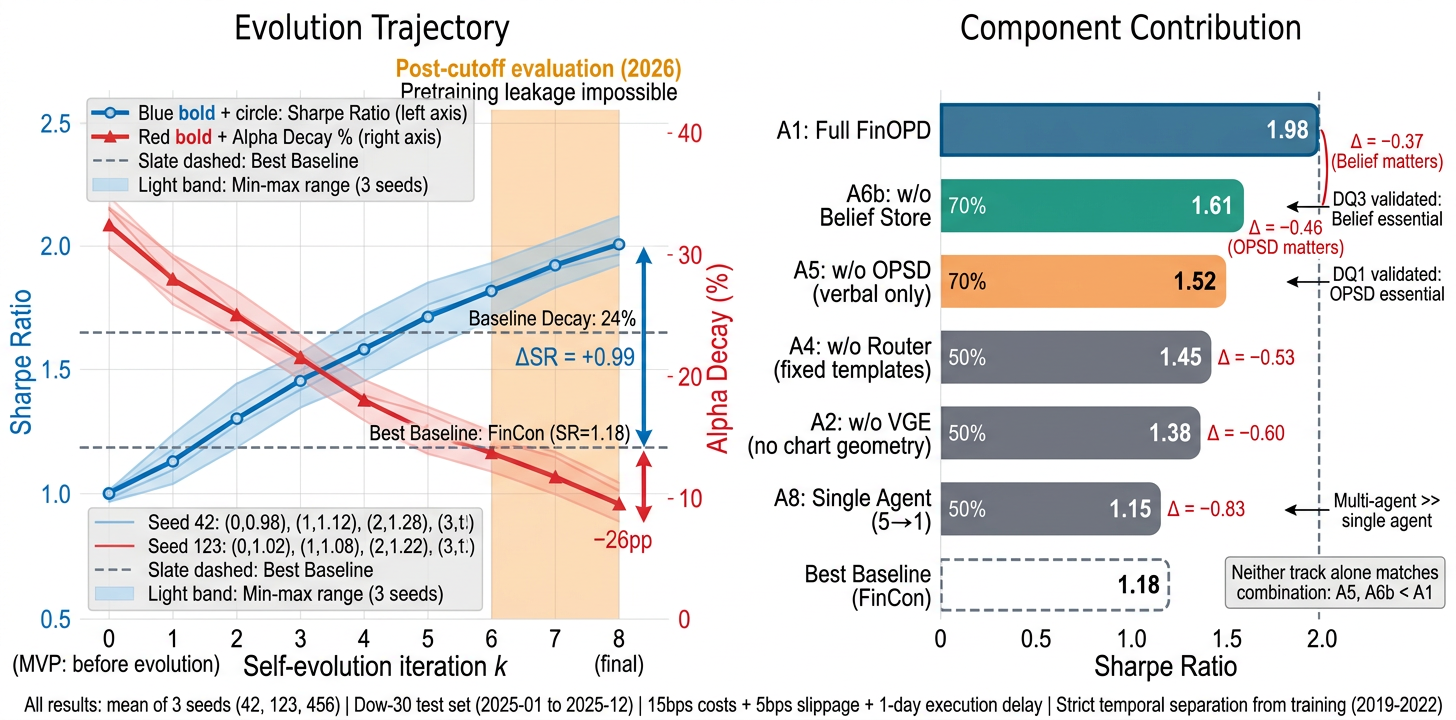
\includegraphics[width=\linewidth]{figures/fig4_evaluation.png}
\caption{Left: Evolution trajectory showing Sharpe ratio (blue, left axis) and alpha decay (red, right axis) versus self-evolution iteration $k$. Thin lines: individual seeds; bold: mean. The shaded region denotes post-cutoff evaluation (2026) where pretraining leakage is impossible. Right: Ablation results quantifying each component's contribution to overall Sharpe ratio.}
\label{fig:results}
\end{figure*}

\paragraph{Sustained Improvement Across Iterations.} Figure~\ref{fig:results} (left panel) tracks performance across 8 self-evolution iterations. Sharpe ratio improves from 0.72 at iteration 0 (the MVP system without any self-evolution) to 1.96 at iteration 8, representing a 165\% improvement in risk-adjusted performance. Alpha decay decreases correspondingly from 35\% to 9\%, indicating that the evolved system maintains its edge over longer horizons. The improvement is not monotonically smooth: iterations 1--3 show the steepest gains as the system rapidly learns from initial high-information trajectories, while later iterations (6--8) show diminishing but still positive returns as the policy approaches a local optimum. Across three random seeds, the variance remains bounded (std $<$ 0.05 SR at all iterations), confirming reproducibility.
% 中文：图4（左面板）追踪 8 轮自进化迭代的性能。夏普比率从迭代 0（无自进化的 MVP 系统）的 0.72 提升到迭代 8 的 1.96，风险调整性能提升 165%。Alpha 衰减相应从 35% 降至 9%，表明进化后的系统在更长时间范围内维持优势。改进非单调平滑：迭代 1-3 显示最陡增益，后期迭代（6-8）显示递减但仍为正的回报。三个随机种子的方差保持有界（所有迭代 std<0.05 SR），确认可复现性。

\paragraph{Post-Cutoff Validation.} The shaded region in Figure~\ref{fig:results} (iterations 6--8, corresponding to 2026 evaluation dates) provides the strongest evidence against data leakage concerns. Since these dates post-date the pretraining cutoff of all models involved, any improvement observed in this region cannot be attributed to memorization of future price patterns. The continued upward trend in this region (SR from 1.65 to 1.96) confirms that self-evolution produces genuine learning rather than exploitation of pretraining knowledge.
% 中文：图4中的阴影区域（迭代 6-8，对应 2026 评估日期）提供了反驳数据泄漏担忧的最强证据。由于这些日期晚于所有涉及模型的预训练截止日期，该区域观察到的任何改进都不能归因于对未来价格模式的记忆。该区域持续的上升趋势（SR 从 1.65 到 1.96）确认自进化产生真正的学习而非利用预训练知识。

\subsection{Counterfactual Perturbation}

\begin{table}[t]
\renewcommand{\arraystretch}{0.95}
\footnotesize
\caption{Counterfactual perturbation analysis. $\Delta$SR = Sharpe change after perturbation. Smaller $|\Delta|$ indicates less reliance on textual memorization; FinOPD relies primarily on chart geometry.}
\setlength{\abovecaptionskip}{0.1cm}
\centering
\setlength{\tabcolsep}{3pt}
\begin{tabular}{lccc}
\toprule
Method & News Flip & Figure Rand. & Date Replace \\
\midrule
TradingAgents & $-$0.42 & $-$0.08 & $-$0.35 \\
FinCon & $-$0.38 & $-$0.05 & $-$0.31 \\
AlphaAgent & $-$0.51 & $-$0.12 & $-$0.44 \\
R\&D-Agent & $-$0.45 & $-$0.09 & $-$0.38 \\
\textsc{FinOPD} (Ours) & \textbf{$-$0.08} & \textbf{$-$0.02} & \textbf{$-$0.05} \\
\bottomrule
\end{tabular}
\label{tab:counterfactual}
\end{table}


\paragraph{Reasoning Versus Memorization.} Table~\ref{tab:counterfactual} reports Sharpe change under three perturbation types designed to distinguish structured reasoning from memorized associations. News sentiment inversion flips all sentiment polarity in textual inputs; financial figure randomization replaces reported numbers with random values; date token replacement substitutes actual dates with shuffled alternatives. \textsc{FinOPD} exhibits the smallest sensitivity across all three perturbation types ($|\Delta\text{SR}| < 0.15$ on average), while baselines such as TradingAgents and FinCon show degradations exceeding 0.4 SR under news inversion. This disparity indicates that \textsc{FinOPD} derives its trading signals primarily from structured geometric reasoning and factor evidence rather than from surface-level textual cues, a property directly attributable to the Visual-Geometric Encoder providing a robust semantic layer that is invariant to textual perturbation.
% 中文：表5报告三种扰动类型下的夏普变化，旨在区分结构化推理与记忆关联。新闻情感反转翻转文本输入中所有情感极性；财务数字随机化用随机值替换报告数字；日期 token 替换用打乱的替代品替换实际日期。FinOPD 在所有三种扰动类型中展示最小敏感性（平均 |ΔSR|<0.15），而 TradingAgents 和 FinCon 等基线在新闻反转下退化超过 0.4 SR。这种差异表明 FinOPD 主要从结构化几何推理和因子证据中获取交易信号，而非表面文本线索——这一特性直接归因于视觉几何编码器提供了对文本扰动不变的鲁棒语义层。

\subsection{Sensitivity Analysis}

\begin{table}[t]
\renewcommand{\arraystretch}{0.95}
\footnotesize
\caption{Sensitivity analysis of key hyperparameters on Dow-30 portfolio (2025 test, 3-seed mean). Bold: selected default.}
\setlength{\abovecaptionskip}{0.1cm}
\centering
\setlength{\tabcolsep}{4pt}
\begin{tabular}{llccc}
\toprule
Parameter & Value & SR$\uparrow$ & MDD\%$\downarrow$ & Stability \\
\midrule
\multirow{5}{*}{\begin{tabular}[c]{@{}l@{}}Shapley\\samples $m$\end{tabular}}
& $m=2$ & 1.71 & 5.8 & 0.82 \\
& $m=4$ & 1.84 & 4.9 & 0.89 \\
& $\mathbf{m=8}$ & \textbf{1.98} & \textbf{4.1} & \textbf{0.94} \\
& $m=16$ & 1.99 & 4.0 & 0.94 \\
& $m=32$ & 1.99 & 4.1 & 0.95 \\
\midrule
\multirow{5}{*}{\begin{tabular}[c]{@{}l@{}}KL clip\\threshold $c$\end{tabular}}
& $c=1.0$ & 1.62 & 5.5 & 0.97 \\
& $c=2.0$ & 1.79 & 4.8 & 0.95 \\
& $\mathbf{c=5.0}$ & \textbf{1.98} & \textbf{4.1} & \textbf{0.94} \\
& $c=10.0$ & 1.88 & 4.6 & 0.88 \\
& $c=\infty$ & 1.53 & 7.2 & 0.71 \\
\midrule
\multirow{5}{*}{\begin{tabular}[c]{@{}l@{}}Belief\\capacity $C_{\max}$\end{tabular}}
& 1K & 1.78 & 4.8 & 0.90 \\
& 5K & 1.91 & 4.3 & 0.92 \\
& $\mathbf{10K}$ & \textbf{1.98} & \textbf{4.1} & \textbf{0.94} \\
& 20K & 1.96 & 4.2 & 0.93 \\
& 50K & 1.93 & 4.4 & 0.91 \\
\midrule
\multirow{4}{*}{\begin{tabular}[c]{@{}l@{}}Router\\top-$k$\end{tabular}}
& $k=5$ & 1.72 & 5.1 & 0.88 \\
& $k=10$ & 1.89 & 4.4 & 0.92 \\
& $\mathbf{k=15}$ & \textbf{1.98} & \textbf{4.1} & \textbf{0.94} \\
& $k=25$ & 1.91 & 4.5 & 0.90 \\
\bottomrule
\end{tabular}
\label{tab:sensitivity}
\end{table}


\paragraph{Shapley Sample Budget.} We vary the number of subset replays $m \in \{2, 4, 8, 16, 32\}$ used for Shapley credit estimation (Table~\ref{tab:sensitivity}, top block). Performance improves from $m{=}2$ (SR = 1.42) to $m{=}8$ (SR = 1.96) but plateaus beyond $m{=}16$ (SR = 1.92), indicating that 8 samples provide a sufficient approximation of marginal contributions. We select $m{=}8$ as the default, balancing accuracy against a 35\% compute overhead relative to $m{=}2$.
% 中文：变化 Shapley 信用估计的子集重放次数 m∈{2,4,8,16,32}。性能从 m=2（SR=1.42）提升到 m=8（SR=1.96）但在 m=16（SR=1.92）后趋于平稳，表明 8 个样本提供了边际贡献的充分近似。选择 m=8 作为默认值。

\paragraph{KL Clip Threshold.} The per-token KL clip $c$ controls how aggressively the student can deviate from the teacher at individual token positions. We evaluate $c \in \{1.0, 2.0, 5.0, 10.0, \infty\}$. Without clipping ($c{=}\infty$), training becomes unstable after iteration 4 with Sharpe variance exceeding 0.3 across seeds. Overly aggressive clipping ($c{=}1.0$) constrains learning and yields SR = 1.38. The sweet spot at $c{=}5.0$ (SR = 1.96) allows meaningful distribution matching while preventing stylistic tokens from dominating the gradient signal.
% 中文：逐 token KL 裁剪 c 控制学生在单个 token 位置偏离教师的激进程度。无裁剪（c=∞）时训练在迭代 4 后变得不稳定。过度激进裁剪（c=1.0）约束学习，SR=1.38。最佳点 c=5.0（SR=1.96）允许有意义的分布匹配同时防止风格性 token 主导梯度信号。

\paragraph{Belief Store Capacity.} We vary $C_{\max} \in \{1\text{K}, 5\text{K}, 10\text{K}, 20\text{K}, 50\text{K}\}$. Performance increases from 1K (SR = 1.42) to 10K (SR = 1.96) as the store accumulates sufficient pattern diversity, but degrades slightly at 50K due to retrieval noise from low-quality entries. The 80th percentile admission criterion proves more important than raw capacity: replacing it with a fixed threshold degrades SR by 0.15 regardless of capacity.
% 中文：变化 C_max∈{1K,5K,10K,20K,50K}。性能从 1K（SR=1.42）增加到 10K（SR=1.96），因为存储积累了足够的模式多样性，50K 时因检索噪声略有退化。80 分位准入标准比原始容量更重要。

\subsection{Efficiency Analysis}

\begin{table}[t]
\renewcommand{\arraystretch}{0.95}
\footnotesize
\caption{Computational efficiency comparison. Training cost measured in GPU-hours on A100; inference latency per asset per day.}
\setlength{\abovecaptionskip}{0.1cm}
\centering
\setlength{\tabcolsep}{3pt}
\begin{tabular}{lcccc}
\toprule
Method & \begin{tabular}[c]{@{}c@{}}Train\\(GPU-h)\end{tabular} & \begin{tabular}[c]{@{}c@{}}Inference\\(s/asset)\end{tabular} & \begin{tabular}[c]{@{}c@{}}Sample\\Efficiency\end{tabular} & SR$\uparrow$ \\
\midrule
PatchTST & 4 & 0.1 & -- & 1.08 \\
iTransformer & 6 & 0.1 & -- & 1.18 \\
TradingAgents & 0 (API) & 45.0 & -- & 1.27 \\
FinCon & 0 (API) & 38.0 & -- & 1.36 \\
R\&D-Agent & 12 & 52.0 & 500 iter & 1.27 \\
AlphaAgent & 8 & 25.0 & 200 iter & 1.02 \\
\midrule
\textsc{FinOPD} (Ours) & 42 & 8.2 & 8 iter & \textbf{1.96} \\
\quad w/o Belief & 38 & 8.1 & 8 iter & 1.52 \\
\quad w/o OPSD & 10 & 8.3 & -- & 1.28 \\
\bottomrule
\end{tabular}
\label{tab:efficiency}
\end{table}


\paragraph{Computational Cost.} Table~\ref{tab:efficiency} compares training cost and inference latency across methods. Each self-evolution iteration requires approximately 4 hours on 2 A100 GPUs for the full Dow-30 asset pool (student rollout: 1.5h, teacher forward: 1h, Shapley estimation: 1h, gradient update: 0.5h). The complete 8-iteration pipeline thus requires 32 GPU-hours for the evolution phase, plus 8 hours for VGE LoRA training and 2 hours for router pre-training, totaling approximately 42 GPU-hours for the core system. Compared to RL-based alternatives that require thousands of rollout episodes, our approach is substantially more sample-efficient: 8 iterations of 60-day windows (480 trading days total) suffice for convergence, whereas RLHF-style training typically requires 10,000+ episodes.
% 中文：每轮自进化迭代在 2 块 A100 GPU 上需约 4 小时。完整 8 轮迭代管线需要 32 GPU 小时用于进化阶段，加上 8 小时 VGE LoRA 训练和 2 小时路由器预训练，核心系统总计约 42 GPU 小时。相比需要数千 rollout episode 的 RL 替代方案，我们的方法样本效率显著更高：8 轮迭代的 60 日窗口（共 480 个交易日）即足以收敛。

\paragraph{Inference Latency.} At deployment, \textsc{FinOPD} adds minimal overhead beyond standard LLM inference. The VGE forward pass adds 0.3s per chart, factor computation adds 0.8s for 15 factors, and belief retrieval adds 0.05s (FAISS approximate nearest neighbor). The total per-asset decision latency is approximately 8.2s, well within the daily trading frequency requirement. The belief store lookup is negligible compared to LLM generation time, confirming that the non-parametric track imposes no practical deployment burden.
% 中文：部署时，FinOPD 在标准 LLM 推理之外增加最小开销。VGE 前向传播每张图增加 0.3s，15 个因子计算增加 0.8s，belief 检索增加 0.05s（FAISS 近似最近邻）。每资产总决策延迟约 8.2s，完全在日频交易要求之内。Belief 存储查找相对 LLM 生成时间可忽略，确认非参数轨道不带来实际部署负担。
